\documentclass[12pt,t]{beamer}
\usepackage{graphicx}
\setbeameroption{hide notes}
\setbeamertemplate{note page}[plain]
\usepackage{listings}

% header.tex: boring LaTeX/Beamer details + macros

% get rid of junk
\usetheme{default}
\beamertemplatenavigationsymbolsempty
\hypersetup{pdfpagemode=UseNone} % don't show bookmarks on initial view


% font
\usepackage{fontspec}
\setsansfont
  [ ExternalLocation = fonts/ ,
    UprightFont = *-regular ,
    BoldFont = *-bold ,
    ItalicFont = *-italic ,
    BoldItalicFont = *-bolditalic ]{texgyreheros}
\setbeamerfont{note page}{family*=pplx,size=\footnotesize} % Palatino for notes
% "TeX Gyre Heros can be used as a replacement for Helvetica"
% I've placed them in fonts/; alternatively you can install them
% permanently on your system as follows:
%     Download http://www.gust.org.pl/projects/e-foundry/tex-gyre/heros/qhv2.004otf.zip
%     In Unix, unzip it into ~/.fonts
%     In Mac, unzip it, double-click the .otf files, and install using "FontBook"

% named colors
\definecolor{offwhite}{RGB}{255,250,240}
\definecolor{gray}{RGB}{155,155,155}

\ifx\notescolors\undefined % slides
  \definecolor{foreground}{RGB}{255,255,255}
  \definecolor{background}{RGB}{24,24,24}
  \definecolor{title}{RGB}{107,174,214}
  \definecolor{subtitle}{RGB}{102,255,204}
  \definecolor{hilit}{RGB}{102,255,204}
  \definecolor{vhilit}{RGB}{255,111,207}
  \definecolor{lolit}{RGB}{155,155,155}
\else % notes
  \definecolor{background}{RGB}{255,255,255}
  \definecolor{foreground}{RGB}{24,24,24}
  \definecolor{title}{RGB}{27,94,134}
  \definecolor{subtitle}{RGB}{22,175,124}
  \definecolor{hilit}{RGB}{122,0,128}
  \definecolor{vhilit}{RGB}{255,0,128}
  \definecolor{lolit}{RGB}{95,95,95}
\fi
\definecolor{nhilit}{RGB}{128,0,128}  % hilit color in notes
\definecolor{nvhilit}{RGB}{255,0,128} % vhilit for notes

\newcommand{\hilit}{\color{hilit}}
\newcommand{\vhilit}{\color{vhilit}}
\newcommand{\nhilit}{\color{nhilit}}
\newcommand{\nvhilit}{\color{nvhilit}}
\newcommand{\lolit}{\color{lolit}}

% use those colors
\setbeamercolor{titlelike}{fg=title}
\setbeamercolor{subtitle}{fg=subtitle}
\setbeamercolor{institute}{fg=lolit}
\setbeamercolor{normal text}{fg=foreground,bg=background}
\setbeamercolor{item}{fg=foreground} % color of bullets
\setbeamercolor{subitem}{fg=lolit}
\setbeamercolor{itemize/enumerate subbody}{fg=lolit}
\setbeamertemplate{itemize subitem}{{\textendash}}
\setbeamerfont{itemize/enumerate subbody}{size=\footnotesize}
\setbeamerfont{itemize/enumerate subitem}{size=\footnotesize}

% page number
\setbeamertemplate{footline}{%
    \raisebox{5pt}{\makebox[\paperwidth]{\hfill\makebox[20pt]{\lolit
          \scriptsize\insertframenumber}}}\hspace*{5pt}}

% add a bit of space at the top of the notes page
\addtobeamertemplate{note page}{\setlength{\parskip}{12pt}}

% default link color
\hypersetup{colorlinks, urlcolor={hilit}}

\ifx\notescolors\undefined % slides
  % set up listing environment
  \lstset{language=bash,
          basicstyle=\ttfamily\scriptsize,
          frame=single,
          commentstyle=,
          backgroundcolor=\color{darkgray},
          showspaces=false,
          showstringspaces=false
          }
\else % notes
  \lstset{language=bash,
          basicstyle=\ttfamily\scriptsize,
          frame=single,
          commentstyle=,
          backgroundcolor=\color{offwhite},
          showspaces=false,
          showstringspaces=false
          }
\fi

% a few macros
\newcommand{\bi}{\begin{itemize}}
\newcommand{\bbi}{\vspace{24pt} \begin{itemize} \itemsep8pt}
\newcommand{\ei}{\end{itemize}}
\newcommand{\ig}{\includegraphics}
\newcommand{\subt}[1]{{\footnotesize \color{subtitle} {#1}}}
\newcommand{\ttsm}{\tt \small}
\newcommand{\ttfn}{\tt \footnotesize}
\newcommand{\figh}[2]{\centerline{\includegraphics[height=#2\textheight]{#1}}}
\newcommand{\figw}[2]{\centerline{\includegraphics[width=#2\textwidth]{#1}}}


%%%%%%%%%%%%%%%%%%%%%%%%%%%%%%%%%%%%%%%%%%%%%%%%%%%%%%%%%%%%%%%%%%%%%%
% end of header
%%%%%%%%%%%%%%%%%%%%%%%%%%%%%%%%%%%%%%%%%%%%%%%%%%%%%%%%%%%%%%%%%%%%%%

% title info
\title{R/qtl: Just barely sustainable}
\author{\href{http://kbroman.org}{Karl Broman}}
\institute{Biostatistics \& Medical Informatics, UW{\textendash}Madison}
\date{\href{http://kbroman.org}{\tt \scriptsize \color{foreground} kbroman.org}
\\[-4pt]
\href{https://github.com/kbroman}{\tt \scriptsize \color{foreground} github.com/kbroman}
\\[-4pt]
\href{https://twitter.com/kwbroman}{\tt \scriptsize \color{foreground} @kwbroman}
\\[2pt]
\scriptsize {\lolit Slides:} \href{http://bit.ly/UseR2016}{\tt \scriptsize
  \color{foreground} bit.ly/UseR2016}
}


\begin{document}

% title slide
{
\setbeamertemplate{footline}{} % no page number here
\frame{
  \titlepage

  \vfill \hfill 
\includegraphics[height=6mm]{Figs/cc-zero.png} \vspace*{-1cm}

  \note{These are slides for a talk that I will give at the UseR 2016
    conference at Stanford on 28 June 2016.

    Source: {\tt https://github.com/kbroman/Talk\_UseR2016} \\
    Slides: {\tt http://bit.ly/UseR2016\_nonotes} \\
    With notes: {\tt http://bit.ly/UseR2016}
}
} }


\begin{frame}[c]{}

\figw{Figs/rqtl_lines_code.pdf}{1.0}

\note{
  Growth of R/qtl over time. Currently about 60\% R code and 40\% C
  code.
}

\end{frame}


\begin{frame}[c]{}

\vspace*{-1mm} \hspace*{-2mm}
\figw{Figs/inbredmice.jpg}{1.2}

\note{
I'll start with a bit of background.

I focus on genetics problems, and particularly on mouse genetics.

I think these are SWR mice; the photo is from David Threadgill.
}

\end{frame}


\begin{frame}{}

\vspace*{18mm}

\centerline{
\begin{minipage}[t]{50mm}
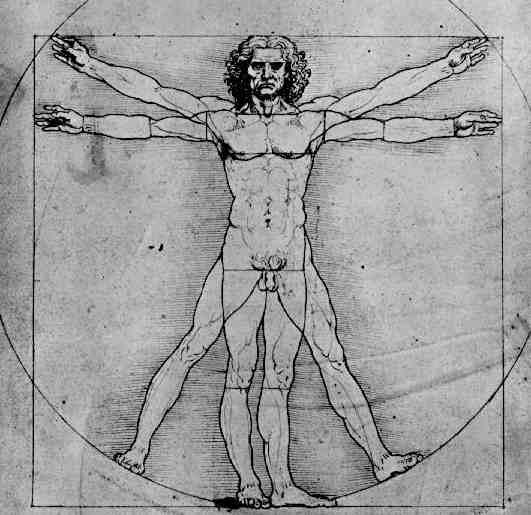
\includegraphics[height=50mm]{Figs/da-vinci-man.jpg}
\end{minipage}
\hspace{15mm}
\begin{minipage}[t]{50mm}
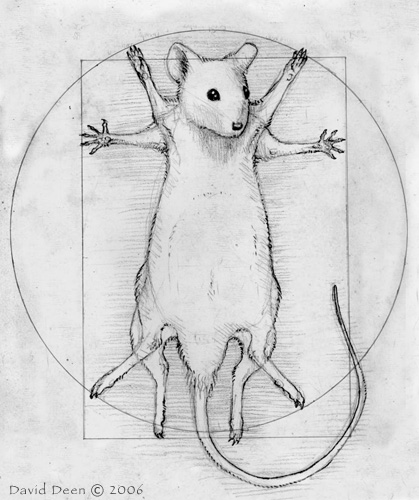
\includegraphics[height=50mm]{Figs/vitruvian_mouse.jpg}
\hspace{5mm}
\href{http://daviddeen.com}{\scriptsize \lolit \tt daviddeen.com}
\end{minipage}
}


\note{
Mice are not humans, but you can learn a great deal about human
biology and disease from mice.

The figure on the right is from David Deen.
}
\end{frame}


\begin{frame}[c]{Intercross}

\figh{Figs/intercross.pdf}{1.0}

\note{
  I've mostly focused on simple crosses between two inbred strains.

  Say strain P$_1$ has low blood pressure and P$_2$ has high blood
  pressure. We cross the two strains to get the F$_1$ hybrid, and then
  intercross F$_1$ siblings to get a large set of F$_2$
  individuals.

  The F$_2$ mice may inherit a P$_1$ or P$_2$ chromosome
  intact, but generally their chromosomes are a mosaic of the two
  parental chromosomes as a result of recombination at meiosis.  The
  points of exchange are called crossovers or recombination events.

  At any one autosomal locus, the F$_2$ individuals will have genotype
  BB, BR, or RR. We'd generate many such mice and then determine their
  genotype along chromosomes as well as measure their phenotype (e.g.,
  blood pressure). The simplest analyis is to look for genomic regions
  where genotype is associated with phenotype.
}
\end{frame}


\begin{frame}[c]{QTL mapping}

\vspace{5mm}
\only<1 | handout 0>{\figh{Figs/lodcurve_insulin.pdf}{0.9}}
\only<2>{\figh{Figs/lodcurve_insulin_with_effects.pdf}{0.9}}

\note{
  Our goal is to identify quantitative trait loci (QTL): regions of
  the genome for which genotype is associated with the phenotype.

  The basic analysis is to consider each locus, one at a time, split
  the mice into the three genotype groups, and perform analysis of
  variance.

  We then plot a test statistic that indicates the strength of the
  genotype-phenotype association.  For historical reasons, we
  calculate a LOD score as the test statistic: the log$_{10}$
  likelihood ratio comparing the hypothesis that there's a QTL at that
  position to the null hypothesis of no QTL anywhere.

  Large LOD scores indicate evidence for QTL and correspond to there
  being a difference in the phenotype average for the three genotype
  groups.
}
\end{frame}


\begin{frame}[c]{R/qtl}

\figw{Figs/rqtl_lines_code.pdf}{1.0}

\note{
  Back to this R/qtl package...
}

\end{frame}


\begin{frame}[c]{Summary}

  \begin{itemize}
  \itemsep12pt
  \item Sustainable software
    \bi
    \item Easier if you are your primary user
    \ei
  \item Take care of your users
    \bi
    \item Answer each question as if it's the first
    \item Primary goal is to be helpful
    \item Write many focused vignettes solving real problems
    \ei
  \item Version control
  \item Tests
  \end{itemize}

  \note{
    It's always good to include a summary.
}
\end{frame}

\begin{frame}[c]{}

\Large

Slides: \href{http://bit.ly/UseR2016}{\tt bit.ly/UseR2016} \quad

\includegraphics[height=5mm]{Figs/cc-zero.png}

\vspace{10mm}

\href{http://kbroman.org}{\tt kbroman.org}

\vspace{10mm}

\href{https://github.com/kbroman}{\tt github.com/kbroman}

\vspace{10mm}

\href{https://twitter.com/kwbroman}{\tt @kwbroman}


\note{
  Here's where you can find me, as well as the slides for this talk.
}
\end{frame}




\end{document}
